% Created 2022-11-23 mié 12:40
% Intended LaTeX compiler: pdflatex
\documentclass[10pt]{article}
\usepackage[utf8]{inputenc}
\usepackage[T1]{fontenc}
\usepackage{graphicx}
\usepackage{grffile}
\usepackage{longtable}
\usepackage{wrapfig}
\usepackage{rotating}
\usepackage[normalem]{ulem}
\usepackage{amsmath}
\usepackage{textcomp}
\usepackage{amssymb}
\usepackage{capt-of}
\usepackage{hyperref}
\usepackage[spanish]{babel}
\usepackage{graphicx,geometry}
\geometry{ a4paper, left=1in, right=1in, top=1in, bottom=1in }
\renewcommand\familydefault{\sfdefault}
\usepackage{sectsty}
\sectionfont{\normalfont\Large }
\subsectionfont{\normalfont\normalsize}
\usepackage{tabularx}
\usepackage{listings}
\lstdefinestyle{mystyle}{
numbers=left,
showspaces=false,
frame=single,
showspaces=false,
showstringspaces=false,
showtabs=false,
numberstyle=\tiny,
aboveskip=\parskip,
basicstyle=\ttfamily\footnotesize
}
\lstset{
style=mystyle,
literate={á}{{\'a}}1
{é}{{\'e}}1
{í}{{\'{\i}}}1
{ó}{{\'o}}1
{ú}{{\'u}}1
{Á}{{\'A}}1
{É}{{\'E}}1
{Í}{{\'I}}1
{Ó}{{\'O}}1
{Ú}{{\'U}}1
{ü}{{\"u}}1
{Ü}{{\"U}}1
{ñ}{{\~n}}1
{Ñ}{{\~N}}1
{¿}{{?``}}1
{¡}{{!``}}1
}
\makeatletter
\usepackage{fancyhdr}
\pagestyle{fancy}
\usepackage{mdframed}
\BeforeBeginEnvironment{minted}{\begin{mdframed}}
\AfterEndEnvironment{minted}{\end{mdframed}}
\author{Luis Eduardo Galindo Amaya (1274895)}
\date{16-11-2022}
\title{Prueba de normalidad}
\hypersetup{
 pdfauthor={Luis Eduardo Galindo Amaya (1274895)},
 pdftitle={Prueba de normalidad},
 pdfkeywords={},
 pdfsubject={},
 pdfcreator={Emacs 26.3 (Org mode 9.1.9)}, 
 pdflang={Spanish}}
\begin{document}


\newcommand{\docente}{Olivia Mendoza Duarte}
\newcommand{\asignatura}{Estadística Avanzada}
\newcommand{\semestre}{2022-2}

\newcommand{\miportada}[1]{
	\begin{titlepage}
		\vspace*{0.75in}
		\begin{flushleft}
			\sffamily
			\large #1       \\
			\Huge
            \@title         \\
			\hrulefill
			\vspace{0.25in} \\
			\Large \@author \\
			%% \vspace*{\fill}
            %% 
\includegraphics[width=\textwidth]{../includes/filler.png} \\
			\vspace*{\fill}
			\large
			\begin{tabular}{|l|l|}
              \hline
			  Asignatura & \asignatura \\
			  Docente    & \docente    \\
			  Fecha      & \@date      \\
              \hline
			\end{tabular}
		\end{flushleft}
	\end{titlepage}
}

\miportada{ Práctica 10 }

\fancyhf{}
\lhead{ \asignatura }
\rhead{ \semestre }
\rfoot{Página \thepage}

\setlength\parindent{0pt}   % eliminar el intentado
\setlength{\parskip}{1.2em}

\maketitle
\end{center}

\section*{Información del dataset\footnote{\url{https://archive-beta.ics.uci.edu/ml/datasets/iris}}}
\label{sec:org1b0370c}
This is one of the best known datasets in statistics and machine learning.  Fisher's paper is a classic in the field and is frequently used for tutorial and teaching purposes. The data set contains 3 classes of 50 instances each, where each class refers to a type of iris plant.  One class is linearly separable from the other 2; the latter are not linearly separable from each other.

Predicted attribute: class of iris plant.

\section*{Desarollo de la práctica}
\label{sec:orgadd281e}
\subsection*{1. Probar el código proporcionado en recursos para la prueba de normalidad, cambiando el número de clases a 5, 6, 8 y 10}
\label{sec:orgab49111}

\begin{figure}[htbp]
\centering
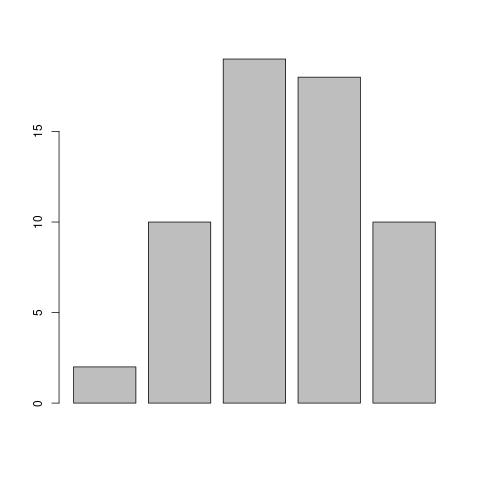
\includegraphics[width=5cm]{img/e1.jpeg}
\caption{5 clases}
\end{figure}

\begin{figure}[htbp]
\centering
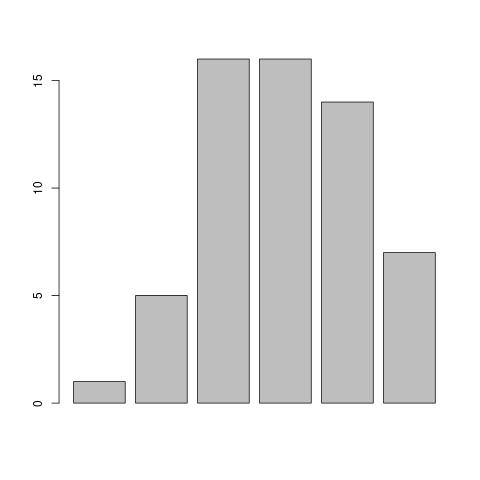
\includegraphics[width=5cm]{img/e2.jpeg}
\caption{6 clases}
\end{figure}

\begin{figure}[htbp]
\centering
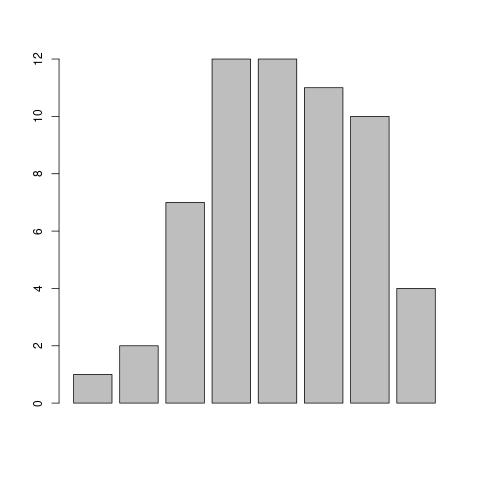
\includegraphics[width=5cm]{img/e3.jpeg}
\caption{8 clases}
\end{figure}

\begin{figure}[htbp]
\centering
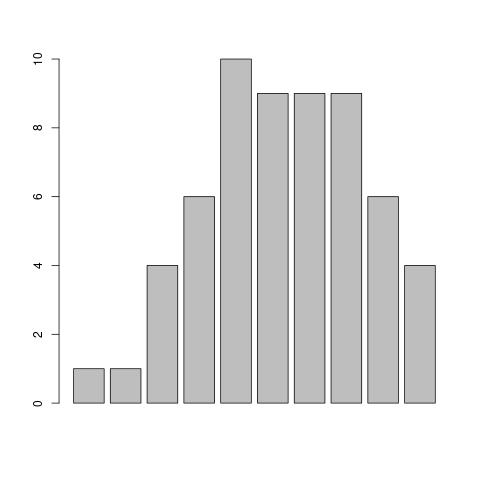
\includegraphics[width=5cm]{img/e4.jpeg}
\caption{10 clases}
\end{figure}

\subsection*{2. Probar este código adaptándolo al menos hasta encontrar alguna que muestre evidencia de distribución normal}
\label{sec:org594c6d0}

Se puede notar como el ancho del sépalo se distribuye de manera normal, el tamaño del sépalo tiende a ser de un tamaño especifico y no tanto del tamaño de los pétalos 

\begin{figure}[htbp]
\centering
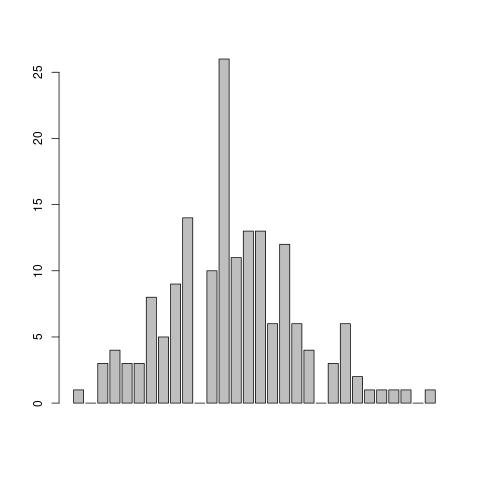
\includegraphics[width=7cm]{img/iris.jpeg}
\caption{columna ''sepal width'' del dataset bezdekIris}
\end{figure}

\subsection*{3. Reportar en un documento todos los resultados obtenidos aún que el comportamiento de los datos no de evidencia de distribución normal}
\label{sec:orgbaa9c33}

El largo del sépalo se distribuye de manera serrada sobre los datos, no parece haber un patrón en la gráfica

\begin{figure}[htbp]
\centering
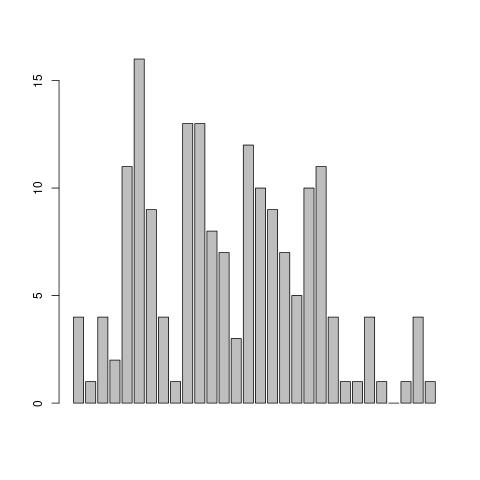
\includegraphics[width=7cm]{img/iris0.jpeg}
\caption{columna ''sepal length'' del dataset bezdekIris}
\end{figure}

Por otro lado el largo de los pétalos es muy interesante, en la parte derecha parece haber una distribución normal pero tiene unos sectores que sobresalen a la izquierda.

\begin{figure}[htbp]
\centering
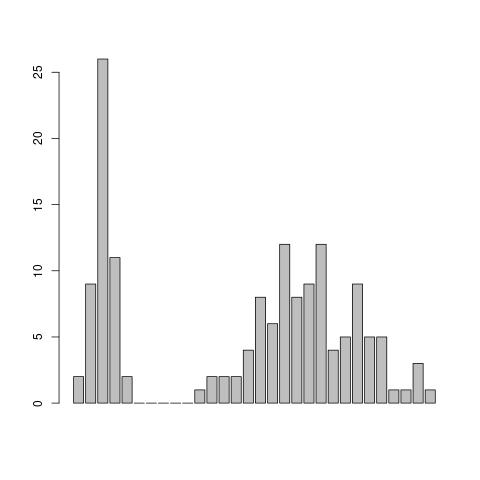
\includegraphics[width=7cm]{img/iris1.jpeg}
\caption{columna ''petal length'' del dataset bezdekIris}
\end{figure}

\pagebreak

\section*{Código}
\label{sec:org61880de}
\lstinputlisting{./pruebaDeNormalidad.R}
\end{document}
